% ARPEGOS:  Automatized Roleplaying-game Profile Extensible Generator Ontology based System %
% Author : Alejandro Muñoz Del Álamo %
% Copyright 2019 %

% Section 5.2: Diseño lógico de Datos %
\section{Diseño Lógico de Datos}
\subsection{Introducción}
En esta sección se va a exponer de forma detallada el proceso de diseño de la ontología que será desarrollada 
para el proyecto. Con este objetivo, se realizará un estudio del diagrama conceptual 
que se muestra en el apartado \ref{Modelo_conceptual}. Este proceso de transformar el esquema del 
modelo conceptual a una estructura lógica que permita almacenar los datos de la aplicación de la 
manera adecuada, se conoce como \textit{diseño lógico}. \medskip

Antes de abordar el proceso, cabe destacar que para poder realizar una ontología que permita comprobar 
que el proyecto puede trabajar con \textit{RPGs} de todo tipo de complejidad, es necesario que el 
juego que se utilice como ejemplo sea lo más completo posible, de manera que juegos de igual o menor   
complejidad puedan ser desarrollados y utilizados asegurando la fiabilidad y completitud de la aplicación. \medskip

Por consiguiente, y tras realizar búsquedas de juegos de rol en base a su complejidad, el equipo de 
desarrollo ha tomado la decisión de utilizar como juego de ejemplo \textit{\textbf{Ánima: Beyond Fantasy}}.
\anima es un juego de rol de mesa que transcurre en un mundo de magia y fantasía, con un sistema
bastante detallado y una complejidad muy elevada, hasta el punto de que hay jugadores que lo evitan 
debido a la larga duración del proceso de creación de personaje, por lo que hace de este juego un caso 
perfecto para demostrar la eficacia de este proyecto.

\subsection{Metodología}
Antes de proceder al desarrollo de la ontología de \anima, se ha considerado fundamental plantear 
que es imposible abordar una fuente de información tan compleja como un \textit{RPG} directamente. En consecuencia, 
el equipo de desarrollo ha procedido a modular el diseño de la ontología, de modo que se aborden los diferentes 
elementos de la ontología por separado, y poco a poco se vayan acoplando hasta que se obtenga el resultado final. \medskip

\subsubsection{Individuos}
Como se ha indicado previamente en el apartado \ref*{Elementos_modelo_conceptual} de la sección \ref*{Modelo_conceptual}, 
un individuo es la \textit{la representacion de un objeto real en el dominio}. Para la elaboración de la ontología de 
\anima, se considerará que un individuo es \textit{la representación de un elemento del dominio, y por tanto, 
tiene una o varias propiedades que lo definen}.

\subsubsection{Clase}
En una ontología, una clase consiste en \textit{un conjunto de individuos que comparten las mismas propiedades y/o 
comportamientos}, tal y como se ha mencionado en el apartado \ref*{Elementos_modelo_conceptual} 
de la sección \ref*{Modelo_conceptual}.

\subsubsection{Propiedades}
La \textit{Real Academia Española} \autocite*{propiedadRAE} define una propiedad como 
\textit{“Atributo o cualidad esencial de alguien o algo”}. Según indica la referencia del 
\textit{OWL Web Ontology Language Reference} \autocite*{Bechhofer2004a}, \textit{OWL} distingue 
dos categorías principales de propiedades:

\begin{itemize}
    \item \textit{\textbf{Datatype properties}}: Las propiedades de tipos de datos conectan individuos con valores de datos.
    \item \textit{\textbf{Object properties}}: Las propiedades de objeto conectan individuos con otros individuos.
\end{itemize}

\subsubsection{Anotaciones}
Como definen Parsia y Kalyanpur \autocite*{Parsia2004}, una anotación es una propiedad que se puede aplicar de manera uniforme a todos los tipos de entidad 
de \textit{OWL}: ontologías, clases, individuos y propiedades. Esta propiedad se considera como un 
comentario, y aunque no pueden definir axiomas, permiten añadir información útil a las entidades pertenecientes 
a cualquier ontología. \medskip

Las anotaciones son un elemento fundamental para el desarrollo de este proyecto, pues posibilitan la introducción de 
información necesaria para algunas entidades de las ontologías, que no pueden o no deben ser indicadas como propiedades 
de las mismas, pues no forman parte de su descripción, sino que aportan información 
imprescindible para el correcto funcionamiento de la aplicación.\medskip

En este proyecto se utilizan diversos tipos de anotaciones, que se podrían separar en dos conjuntos:
\begin{itemize}
    \item \textit{\textbf{Standard annotations}}: Consideramos anotaciones estándar a aquellas que permiten introducir 
    información extra a cualquier entidad de la ontología, incluyendo a esta última también. Son anotaciones que están 
    definidas previamente. Este conjunto esta formado por las siguientes anotaciones:

    \begin{itemize}
        
        \item \textit{rdfs:comment}: Esta anotación se utilizará como descripción de las entidades a las que se vincula, por lo que 
        deberá contener la referencia completa de información del elemento al que hace alusión. El tipo de dato asociado debe ser 
        \textbf{xsd:string}.

        \item \textit{rdfs:IsDefinedBy}: Esta anotación permite indicar qué elemento indica o define el valor 
        de la entidad a la que está asociada. Sólo debe contener el nombre de dicho elemento con el tipo de dato \textbf{xsd:string}.
    \end{itemize}

    \item \textit{\textbf{Stage annotations}}: Las anotaciones de etapa son anotaciones definidas por el equipo de desarrollo 
    para poder aportar la información necesaria para determinar qué entidades se pueden considerar como \textit{etapas de creación}, 
    y de qué manera deben ser procesadas. Toda ontología que pertenezca a este proyecto deberá disponer de ellas adecuadamente para 
    definir las etapas de creación de un personaje. A continuación se indica cuales son:

    \begin{itemize}
        \item \textit{CreationScheme}: Esta anotación describe cuál es el esquema de creación de un personaje. Debe contener 
        de manera ordenada las diversas etapas por las que debe pasar el usuario para crear su personaje. Esta anotación 
        debe ubicarse en cada individuo de la etapa raíz del proceso de creación, utilizando el tipo de dato \textbf{xsd:string}.

        \item \textit{CreationSchemeRoot}: Esta anotación indica qué clase representa la etapa raíz del proceso de creación. 
        Debe estar ubicada en el individuo de la clase \textit{\textbf{ClassDefinition}} correspondiente a la etapa raíz del 
        proceso de creación, y debe tener asociado el valor booleano \textbf{true}.

        \item \textit{GeneralCostDefinedBy}: Esta anotación permite indicar qué elemento define el valor máximo de 
        puntos de una o varias etapas. Debe ser asociada al individuo de la clase \textit{\textbf{ClassDefinition}} correspondiente 
        a la etapa de creación que así lo requiera. Se utiliza de la misma forma que la anotación \textit{rdfs:IsDefinedBy}.

        \item \textit{SubstageOrder}: Esta anotación indica a las etapas que lo requieran, en qué posición se debe mostrar. 
        Normalmente se utiliza en etapas que formen parte de una etapa más general, siendo aplicada al individuo de la clase 
        \textit{\textbf{ClassDefinition}} correspondiente. Su valor debe ser númerico 
        y estar acompañado del tipo de datos \textbf{xsd:unsignedInt}
        
        \item \textit{ValuedListInfo}: Esta anotación debe contener toda la información necesaria para que una etapa de creación 
        que requiera de la vista de introducción de valores realice los cálculos de la manera adecuada. Debe estar asociada 
        al individuo de la clase \textit{\textbf{ClassDefinition}} correspondiente, y debe utilizar el tipo de datos \textbf{xsd:string}.
        
        \item \textit{ViewType}: Esta anotación indica el tipo de vista que debe mostrar la interfaz gráfica de la aplicación 
        cuando se muestre la etapa a la que está vinculada. Debe estar asociada al individuo de la clase 
        \textit{\textbf{ClassDefinition}} correspondiente, y debe indicar el nombre exacto del tipo de vista utilizando
        el tipo de datos \textbf{xsd:string}.
        
    \end{itemize}
\end{itemize}


\subsubsection{Etapas de creación}
Uno de los objetivos del proyecto es que a la hora de crear el personaje, el usuario pueda conocer de forma clara los 
pasos que requiere el juego para crear el personaje de la forma más completa posible. A estos pasos los llamaremos 
\textit{etapas de creación}.\medskip

Para poder definir las etapas de creación de \anima, se han planteado las siguientes preguntas:

\begin{enumerate}
    \item ¿Cuáles son las etapas de creación de personajes del \anima?
    \item ¿Se pueden dividir esas etapas en subetapas más pequeñas?
    \item ¿Cuál debe ser la etapa inicial del proceso de creación?
    \item ¿Son necesarias todas las etapas de creación para cada personaje?
    \item ¿Qué tipo de interacción debe tener el usuario con cada etapa?
\end{enumerate}

La primera respuesta suele encontrarse en los libros de los juegos de rol, ya que es una información 
fundamental para poder crear los personajes. Así sucede en el caso de \anima, de manera que 
echando un ojo rápido al libro, podemos saber que las etapas de creación de un personaje en \anima
son las siguientes: \medskip

\begin{figure}[H]
    \centering
    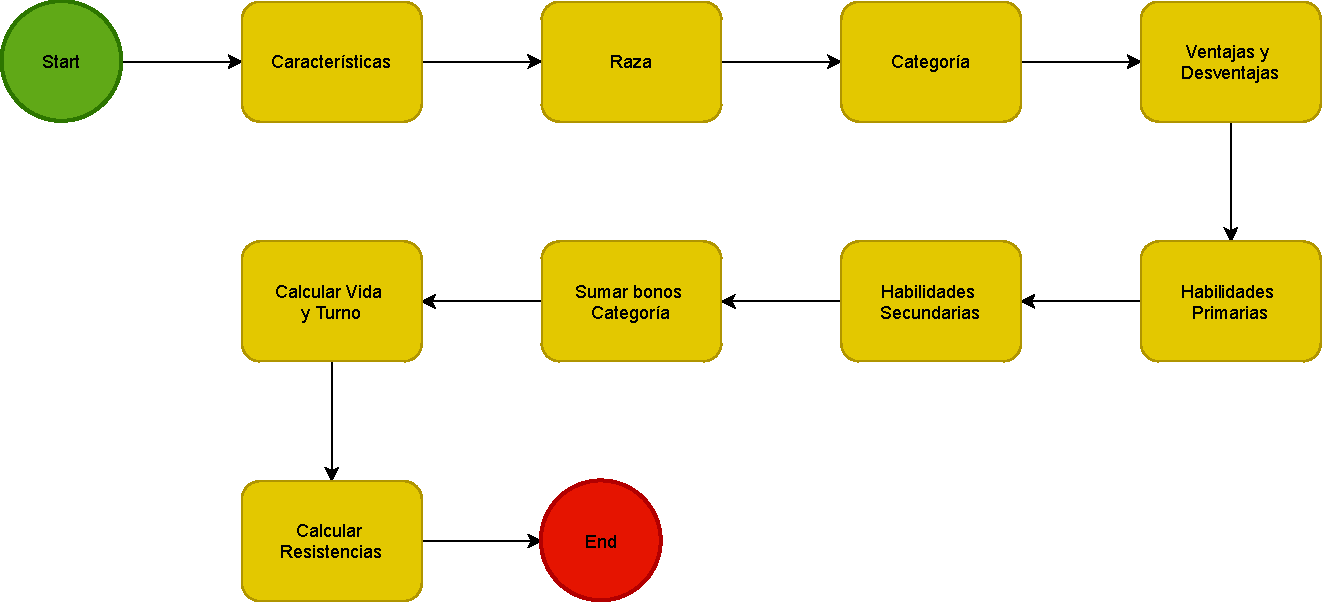
\includegraphics[scale=0.5]{Documentation-Scheme/Desarrollo/Diseño-Sistema/Etapas_Anima.pdf}
    \caption{Etapas de creación de \textit{Ánima: Beyond Fantasy}}
    \label{Etapas_anima}
\end{figure}

Aunque el proceso aparenta ser rápido y sencillo en un principio, cabe recordar que \anima es conocido 
entre los jugadores de rol por su gran complejidad en la creación de personajes, llegando al punto de frustrar a 
los jugadores debido a la inmensidad de información necesaria para completar el personaje. En consecuencia, se 
ha considerado inviable abordar el proceso de creación de forma directa, y se ha planteado modular el proceso en 
un mayor número de etapas, que sean más sencillas e intuitivas. Así, el equipo de desarrollo considera 
\textbf{preferible un proceso largo de etapas sencillas} a un proceso corto de etapas complejas. \medskip

Después de investigar sobre el juego en profundidad, el equipo de desarrollo ha desglosado las etapas de 
creación de personajes de \anima en subetapas que pueden ser mostradas en una única vista y que 
facilitan una interacción intuitiva por parte de los usuarios, y por consiguiente, 
serán las \textbf{etapas de creación} de nuestra aplicación. El diagrama de flujo resultante se puede 
observar en la figura \ref*{Diagrama_creacion_anima} \footnote[1]{Se adjunta una versión ampliada como anexo 
para poder leer el diagrama adecuadamente.}.\medskip

Durante la investigación sobre el juego se observa que hay diferentes tipos de personajes, definidos por 
reglas y que presentan una lista de propiedades y habilidades a las que pueden tener acceso. En \anima, 
a estos tipos se les conoce como \textit{Categorías}. En consecuencia, la \textit{Categoría} de un personaje 
determinará las etapas de creación del mismo y es por esto que el primer elemento del proceso deberá ser 
la elección de \textit{Categoría}. \medskip

Una vez conocemos el orden y las etapas de creación de un personaje, falta saber cómo puede interactuar el usuario 
con cada etapa, pues cada una de ellas puede requerir un tipo de acción diferente por parte del usuario. Además, 
cada juego dispone de etapas diferentes, lo que hace inviable diseñar una vista para la interacción de cada etapa 
de cada juego. \medskip

La propuesta del equipo de desarrollo para salvar este obstáculo consiste en \textbf{generalizar los tipos de interacción} que pueden 
requerir las etapas de creación de cualquier juego. Esto permite diseñar sólo una vista por cada tipo de interacción, y posteriormente 
vincular cada etapa con el tipo de interacción más adecuado. En el caso de \anima, se han contemplado los siguientes 
tipos de interacción: 

\begin{itemize}
    \item \textit{\textbf{Selección única}}: El usuario sólo necesita elegir una opción de todas las disponibles.
    \item \textit{\textbf{Selección múltiple}}: El usuario puede elegir varias opciones de todas las disponibles. 
    Este caso tiene varias posibilidades:
    \begin{itemize}
        \item \textit{Coste estático}: Todas las opciones tienen el mismo coste, y en caso de estar agrupados, no es necesario 
        realizar gasto alguno de puntos para poder seleccionar elementos de un grupo.
        \item \textit{Coste estático y de grupo}: Todos las opciones tienen el mismo coste, y en caso de estar agrupados, poder 
        optar a seleccionar elementos de un grupo hay que pagar un coste.
        \item \textit{Coste dinámico}: Cada opción tiene un coste diferente.
    \end{itemize}
    \item \textit{\textbf{Introducción de valores}}: El usuario debe introducir valores en los elementos mostrados.
\end{itemize}\medskip

Después de apreciar estos posibles casos, se han revisado otros posibles \textit{RPGs} para comprobar que los tipos de 
interacción previamente indicados son reutilizables para otros juegos, y por tanto, convenientes para el desarrollo del 
presente proyecto. \newpage

\begin{figure}
    \centering
    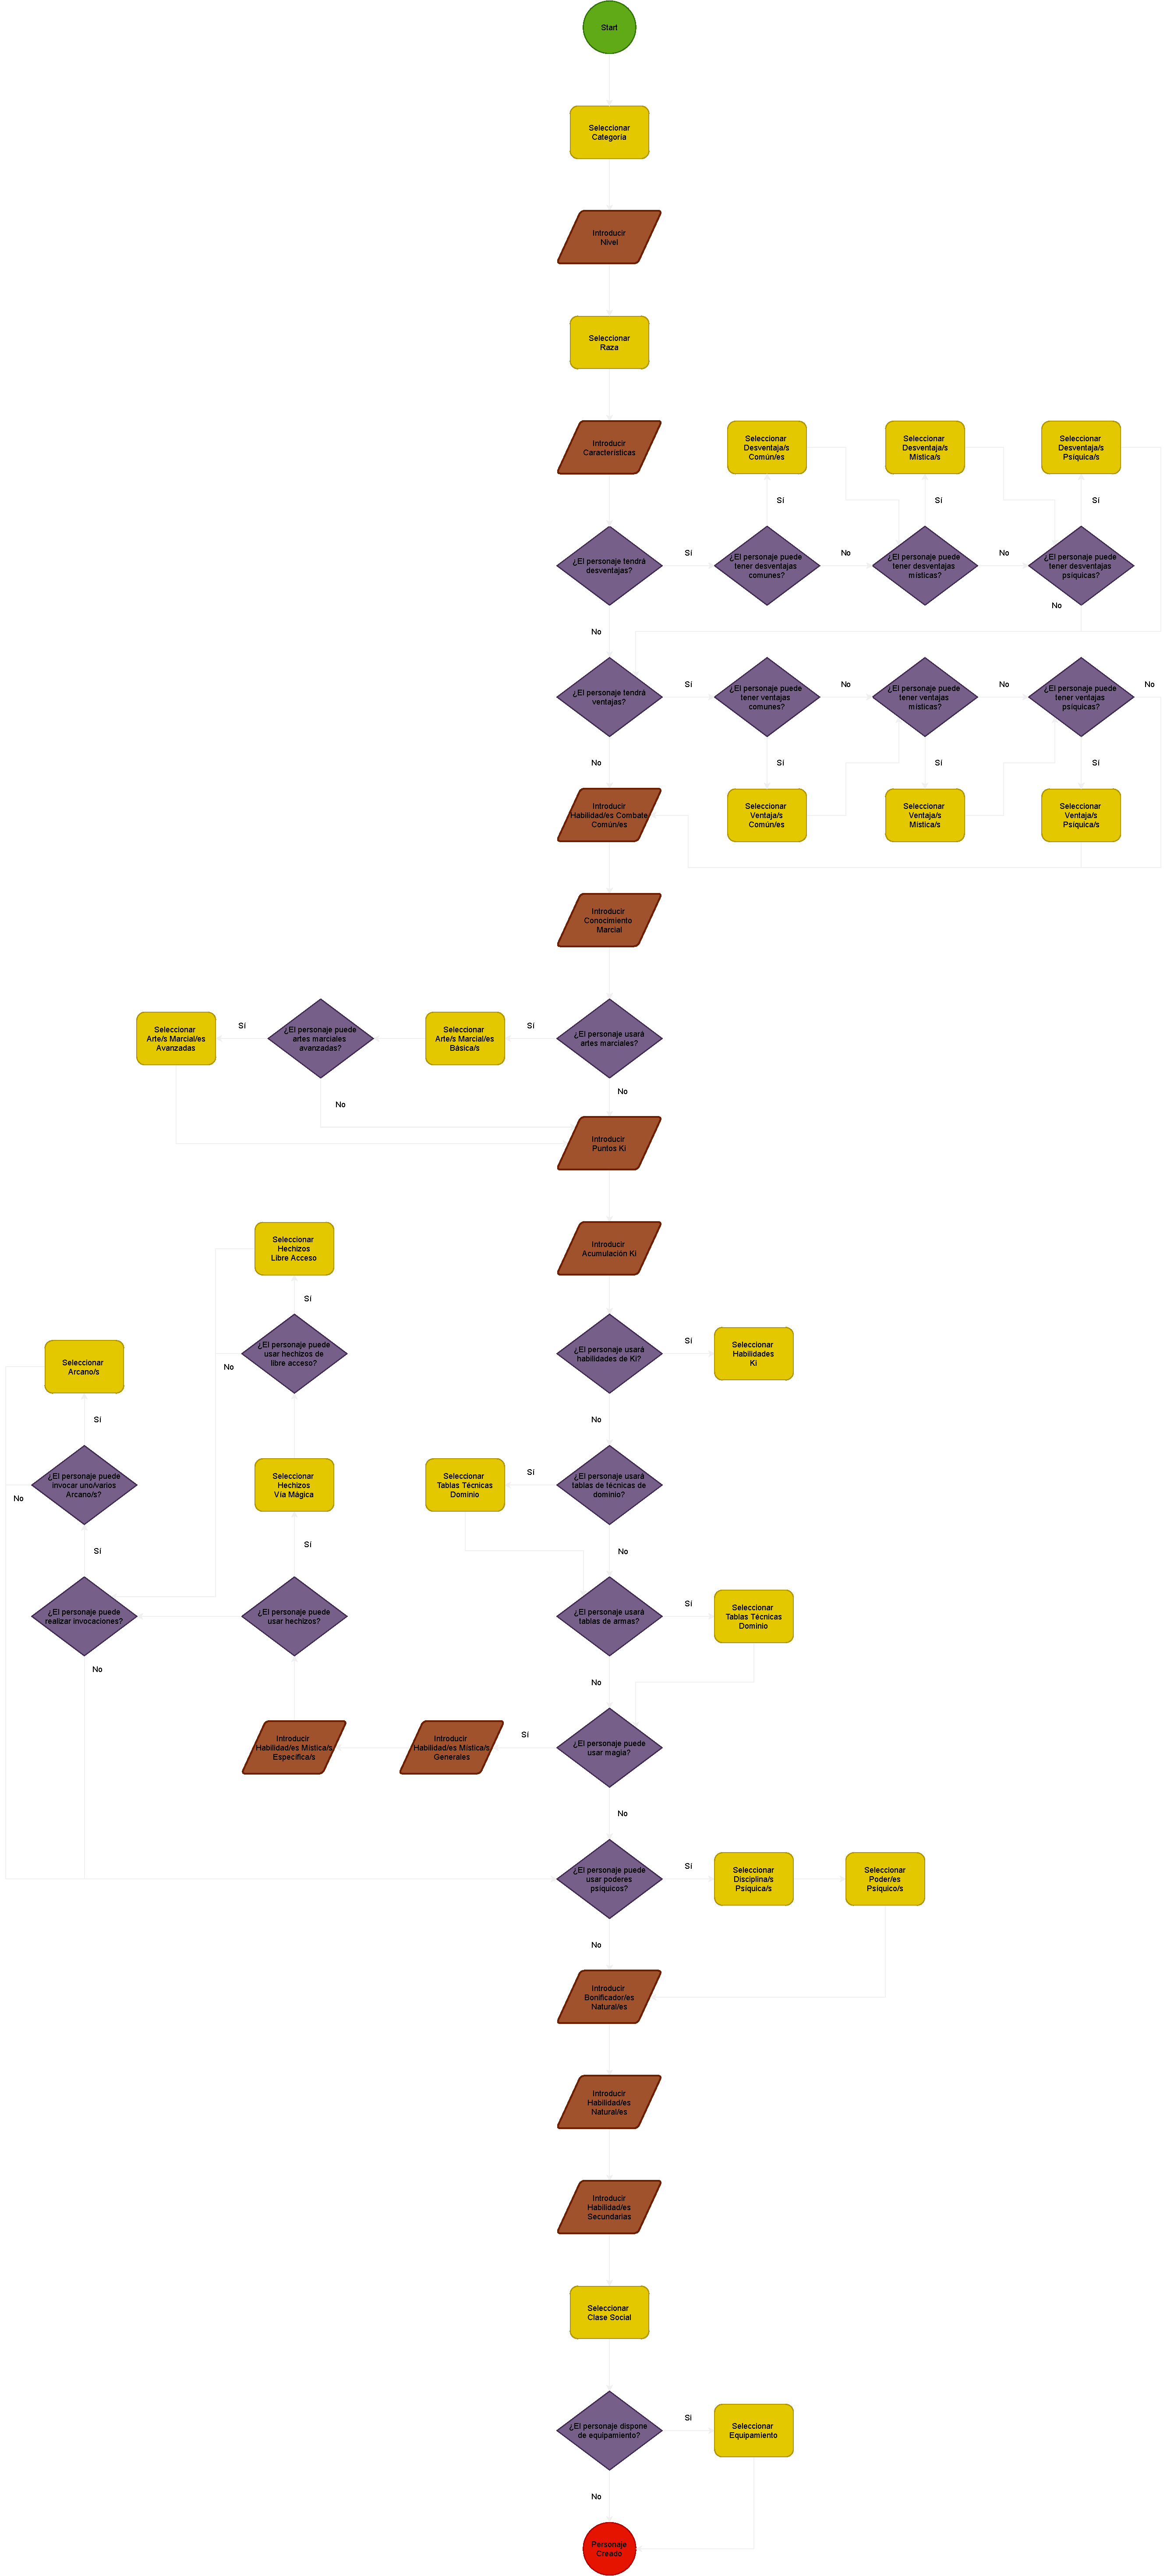
\includegraphics[scale=0.18]{Documentation-Scheme/Desarrollo/Diseño-Sistema/Proceso_Creación_Anima.pdf}
    \caption{Proceso de Creación de \textit{Ánima: Beyond Fantasy}}
    \label{Diagrama_creacion_anima}
\end{figure}
